\chapter{Diseño y arquitectura}\label{cap:diseno}\label{ap:diseno-detallado}

Este capítulo describe cómo se diseñó SavePoint para cumplir los requisitos del
Capítulo~\ref{cap:analisis}. Presenta primero la arquitectura de la plataforma web y las
decisiones que la sostienen, el modelo de datos, la API y la interfaz; después, el diseño de
los algoritmos de recomendación que se construyen sobre ella y del laboratorio que los evalúa.
Plataforma y algoritmos se diseñaron como un único sistema: la aplicación recoge y gobierna las
señales que los algoritmos consumen, mientras que el laboratorio los compara sobre la misma base
de datos y el mismo modelo de dominio.

\section{Arquitectura del sistema}\label{sec:web-diseno}\label{sec:dis-arquitectura}

SavePoint es un monolito modular con dos ejecutables. El backend, en \texttt{apps/api/}, usa
Django~\cite{django} con soporte a largo plazo (LTS) y Django REST Framework (DRF)~\cite{drf} sobre
PostgreSQL~\cite{postgresql}, con el mapeo objeto-relacional (ORM) de Django como interfaz de
persistencia; sus módulos se separan por dominio (\texttt{catalogue}, \texttt{library},
\texttt{accounts}, \texttt{recommendations}, \texttt{evaluation}, \texttt{social},
\texttt{audit}), pero comparten despliegue y base de datos. El frontend, en
\texttt{apps/web/}, es una aplicación Next.js~\cite{nextjs} con React~\cite{react} y
TypeScript en modo estricto, que renderiza en el servidor (SSR) las páginas de solo lectura; el navegador
solo habla con Next.js, que reenvía las llamadas al backend (Sección~\ref{sec:dis-sesion}). Los
trabajos de recomendación y evaluación se
ejecutan como comandos fuera de la petición HTTP: la aplicación publica sus resultados, pero no
vuelve a calcular los resultados de la evaluación en el navegador. La Figura~\ref{fig:arquitectura}
representa esta arquitectura por capas, y el registro de decisión ADR-001 recoge el contexto
completo de esta elección.

\begin{figure}[H]
    \centering
    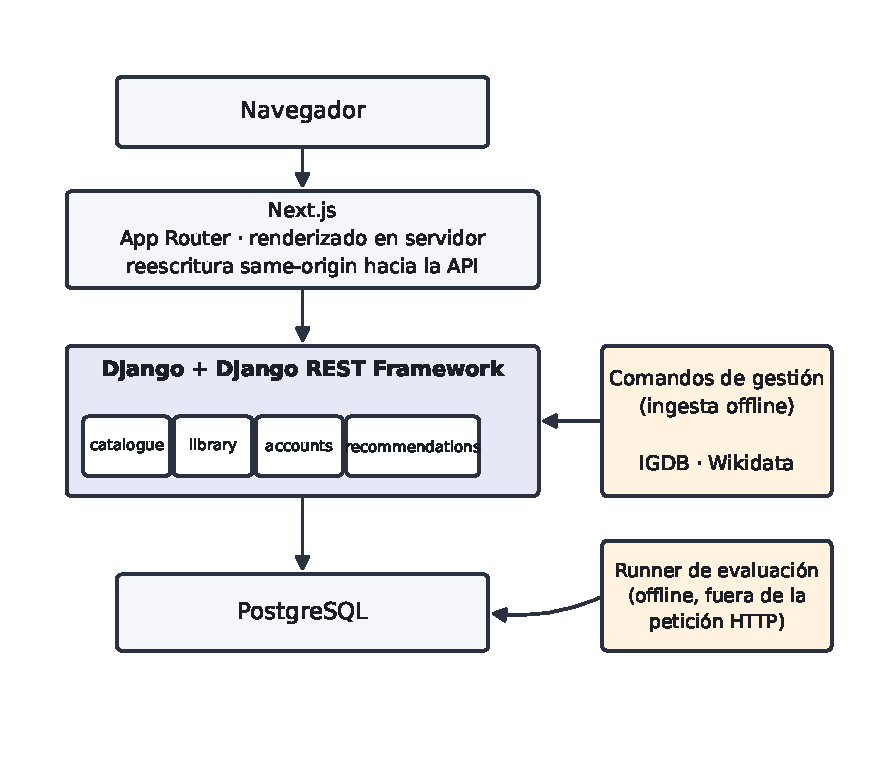
\includegraphics[width=0.8\textwidth]{figures/arquitectura.pdf}
    \caption{Arquitectura de SavePoint: el navegador solo habla con Next.js, que reescribe las llamadas hacia Django y DRF; los comandos de ingesta y el runner de evaluación escriben en PostgreSQL fuera de la petición HTTP.}
    \label{fig:arquitectura}
\end{figure}

Esa elección no fue automática. El dominio de SavePoint (obras, ediciones, copias,
valoraciones, biblioteca) es relacional y con mucha escritura estructurada, el tipo de
problema para el que Django y su ORM están pensados desde el principio, con autenticación,
migraciones y validación ya resueltos en el propio marco de trabajo.
Frente a alternativas más ligeras como FastAPI con SQLAlchemy, que habrían obligado a componer
esas mismas piezas a mano, Django ofrece esa base madura sin coste adicional. Frente a servir
la interfaz con plantillas de Django y HTMX, que habría evitado duplicar el contrato de datos
entre backend y frontend, se prefirió un frontend Next.js separado porque el catálogo,
la biblioteca y las recomendaciones necesitaban una interfaz más rica de lo que las plantillas del
lado del servidor ofrecen con comodidad, sin perder por ello el renderizado en servidor que la
accesibilidad y el primer pintado rápido piden. Una arquitectura de microservicios, por
último, se descartó por su coste operativo y de trazabilidad en un proyecto de un único
desarrollador: separar servicios solo se justifica cuando hay una necesidad medida que lo
pida, no por anticipado.

PostgreSQL es la única base de datos de aplicación y de pruebas de integración, en desarrollo,
en pruebas y en despliegue, sin sustituir nunca por una base más ligera en ningún entorno. El
registro ADR-002 explica por qué: el modelo de datos de SavePoint depende de restricciones de
unicidad, de transacciones y de búsqueda por similitud de texto que SQLite soporta de forma
incompleta y que una base documental como MongoDB no ofrece con la misma garantía de
integridad relacional. Usar SQLite en local y PostgreSQL en producción, la solución más
barata a corto plazo, se descartó explícitamente porque introduce una asimetría entre entornos
que un banco de pruebas reproducible no se puede permitir: una consulta que funciona en SQLite
y falla en PostgreSQL, o viceversa, sería un defecto del propio diseño experimental, no del
código. Todo el sistema se levanta, en consecuencia, con Docker Compose a partir de los tres
componentes de aplicación (base de datos, API y frontend), cada uno construido desde su propio
fichero de Docker con versiones de dependencias fijadas; junto a ellos, Compose orquesta además un contenedor de \textit{worker} independiente por cada
variante de recomendación que la web publica (Sección~\ref{sec:alg-publicadas}), y no por las
dieciséis que compara el laboratorio. Un trabajo cuyo objeto
de estudio es la reproducibilidad de una comparación de algoritmos necesita, antes que nada,
que el propio entorno de ejecución sea reproducible, y los contenedores eliminan esa variable
en cualquier máquina que lo levante.

Para el despliegue público se adoptó una topología repartida entre tres proveedores
gratuitos (Vercel para el frontend, Render para el backend y Neon para PostgreSQL), por una
restricción de partida no negociable: coste cero, sin tarjeta de pago. La
Sección~\ref{cap:despliegue}, en el capítulo de implementación, desarrolla esta topología,
sus límites conocidos y el estado actual del despliegue; el registro ADR-005 recoge la
decisión completa.

\section{Decisiones de arquitectura}\label{sec:dis-adr}

Cada decisión de diseño con consecuencias materiales queda registrada en \texttt{docs/adr/}
como registro de decisión de arquitectura (ADR), con un formato fijo de contexto, alternativas,
decisión, evidencia, consecuencias, reversibilidad y aprobación. La
Tabla~\ref{tab:adr-resumen} resume el conjunto vigente; las secciones correspondientes citan
cada registro donde es relevante. Cada registro es citable y reversible: los límites de dominio
y las migraciones actúan como puntos de salida si una decisión se revisa.

\begin{table}[H]
\centering
\begin{tabularx}{\textwidth}{ | >{\raggedright\arraybackslash}p{0.14\textwidth} | Y | }
    \hline
    \textbf{Registro} & \textbf{Decisión y consecuencia principal} \\
    \hline
    ADR-001 & Monolito modular Django/DRF con frontend Next.js separado. Integridad y autenticación maduras, límites de dominio legibles, dos ejecutables con una sola arquitectura operable. \\
    \hline
    ADR-002 & PostgreSQL 18.6 como única base de datos de aplicación y de pruebas de integración. Paridad entre entornos, integridad relacional, bloqueos y búsqueda de trigramas disponibles de forma reproducible. \\
    \hline
    ADR-003 & Corpus congelado de Wikidata bajo dominio público y revisión de Commons por archivo. Evaluación repetible y procedencia visible, sin ninguna consulta a proveedores en tiempo de petición. \\
    \hline
    ADR-004 & Sesión de Django y frontera del mismo origen. Las primitivas de sesión y de protección contra falsificación de petición en sitios cruzados las mantiene Django; ningún token accesible al código del navegador. \\
    \hline
    ADR-005 & Docker Compose local y despliegue público repartido entre tres servicios gratuitos (Vercel, Render y Neon). Coste cero sin tarjeta, a cambio de que el frontend público no sea la misma imagen que la local. \\
    \hline
    ADR-006 & IGDB como fuente del catálogo a escala real, con portadas por enlace directo. Cobertura real y modelado de género y plataforma de primera clase, a cambio de una obligación de atribución continua y de una licencia que es un acuerdo, no una dedicación al dominio público. \\
    \hline
    ADR-007 & Heurístico determinista de afinidad por géneros para la página de recomendaciones. Entrega el requisito como página real y explicable, deliberadamente al margen de la comparación sistemática de recomendadores que la Sección~\ref{cap:algoritmos} presenta más adelante. \\
    \hline
    ADR-008 & Ratings externos gobernados por snapshot versionado, con enriquecimiento acotado desde RAWG. \\
    \hline
    ADR-009 & Familias de algoritmos de recomendación y su ejecución como \textit{workers} aislados. La web publica solo tres de las dieciséis variantes. \\
    \hline
\end{tabularx}
\caption{Registros de decisión de arquitectura vigentes.}
\label{tab:adr-resumen}\label{tab:adr}
\end{table}

\section{Modelo de datos, API y sesión}\label{sec:dis-modelo-datos}\label{sec:dis-api}\label{sec:dis-sesion}\label{sec:dis-frontera}

El modelo de datos, descrito en la Sección~\ref{sec:req-informacion}, sigue cuatro decisiones
de diseño. La primera es que toda identidad canónica es un identificador único universal
(UUID) interno, generado en la importación, con el identificador del proveedor guardado solo
como procedencia; así, cambiar de proveedor o prescindir de él nunca obliga a renumerar el
catálogo (ADR-006, CAT-04). La segunda es que las restricciones y las transacciones viven
también en la base de datos, no solo en la capa de aplicación: unicidad de entrada por
persona y obra, unicidad de copia por clave de idempotencia, rango de la valoración por
restricción de comprobación y un disparador que impide que el cursor de importación de IGDB
retroceda. La tercera es la desnormalización deliberada de la fecha de primer lanzamiento y
de la valoración agregada sobre la propia obra, para que el filtrado por año y por nota sea
un recorrido de índice y no una agregación sobre cientos de miles de publicaciones. La cuarta
es un índice de trigramas sobre los alias normalizados, que sostiene la búsqueda tolerante
por prefijo y por similitud.

La API es de estilo REST, servida por DRF bajo el prefijo \texttt{/api/}. Las respuestas de
lista están paginadas. Las vistas de escritura y las de datos personales exigen sesión. Las
anónimas de mayor coste llevan un límite de ritmo con ámbito propio. La
Tabla~\ref{tab:endpoints} recoge los puntos de acceso principales.

\begin{table}[H]
\centering
\begin{tabularx}{\textwidth}{ | Y | Y | Y | }
    \hline
    \textbf{Método y ruta} & \textbf{Acceso} & \textbf{Función} \\
    \hline
    \path{GET /api/catalogue/games/} & Anónimo & Lista paginada con búsqueda, filtros, orden y facetas. \\
    \hline
    \path{GET /api/catalogue/games/<slug>/} & Anónimo & Ficha de una obra con su jerarquía y su procedencia. \\
    \hline
    \path{GET /api/catalogue/sources/} & Anónimo & Dataset, licencia, hash y política de portadas. \\
    \hline
    \path{POST /api/accounts/login/}, \path{logout/} & Anónimo & Inicio y cierre de sesión con protección de origen. \\
    \hline
    \path{POST /api/accounts/register/} & Anónimo & Registro de nuevas personas usuarias, con límite de ritmo. \\
    \hline
    \path{GET /api/accounts/profiles/<alias>/} & Sesión & Perfil de un amigo aceptado, por lista de campos permitidos. \\
    \hline
    \path{GET /api/library/entries/} & Sesión & Biblioteca de la persona autenticada. \\
    \hline
    \path{POST /api/library/entries/<id>/status/}, \path{rating/}, \path{copies/} & Sesión & Cambio de estado, valoración y alta de copias. \\
    \hline
    \path{GET /api/library/popularity/} & Anónimo & Baseline de popularidad a partir de las señales importadas de IGDB. \\
    \hline
    \path{GET /api/recommendations/genre-taste/} & Sesión & Recomendación por afinidad de géneros de la persona autenticada. \\
    \hline
\end{tabularx}
\caption{Puntos de acceso principales de la API.}
\label{tab:endpoints}
\end{table}

La proyección de un perfil que ve un amigo se construye con una lista explícita de campos permitidos,
escrita a mano, en lugar de una serialización automática por introspección del modelo. Así,
exponer un campo privado nuevo requiere una decisión explícita, que es el modo de fallo
opuesto al de ocultarlo por olvido.

La autenticación sigue el diseño del registro ADR-004. Django emite y valida la sesión. El
navegador solo llama a rutas del mismo origen de Next.js, que las reescribe hacia el backend
mediante una variable de entorno visible únicamente en el servidor. Las cookies de sesión y
de protección contra falsificación de petición en sitios cruzados (CSRF) viajan con ámbito
del mismo origen, sin necesidad de compartir recursos entre orígenes con credenciales. Las
mutaciones exigen el testigo CSRF. El cierre de sesión la invalida. Los redirectos
posteriores al acceso solo aceptan rutas relativas del mismo sitio, revalidadas en el
servidor. No hay ningún testigo de tipo \textit{bearer} accesible al código JavaScript del
navegador.

El diseño mantiene dos fronteras explícitas. Ninguna cuenta es pública, de modo que solo los
amigos aceptados acceden a su contenido, y el acceso a IGDB está confinado a un comando de
gestión fuera de línea, sin que ninguna petición de usuario llame a un proveedor externo
(RN-8 y RN-9 de la Tabla~\ref{tab:reglas-negocio}).

\section{Diseño de la interfaz de usuario}\label{sec:dis-ui}

El diseño de la interfaz se fijó en un contrato de diseño, \texttt{01.1-UI-SPEC.md},
aprobado antes de implementar y validado por un subagente comprobador. El contrato define un
sistema de tokens de variables CSS, con juegos completos para tema claro y tema oscuro, cuya
selección se aplica en el servidor mediante una cookie para evitar el destello al cargar. Los
componentes reutilizables incluyen la tarjeta de juego, las píldoras de estado y de nota, la
valoración por estrellas, la imagen de portada con su marcador de reserva, la barra de
filtros, el conmutador de tema y el selector de cuenta. Las Figuras~\ref{fig:ui-claro}
y~\ref{fig:ui-oscuro} muestran la página de inicio en ambos temas.

\begin{figure}[H]
    \centering
    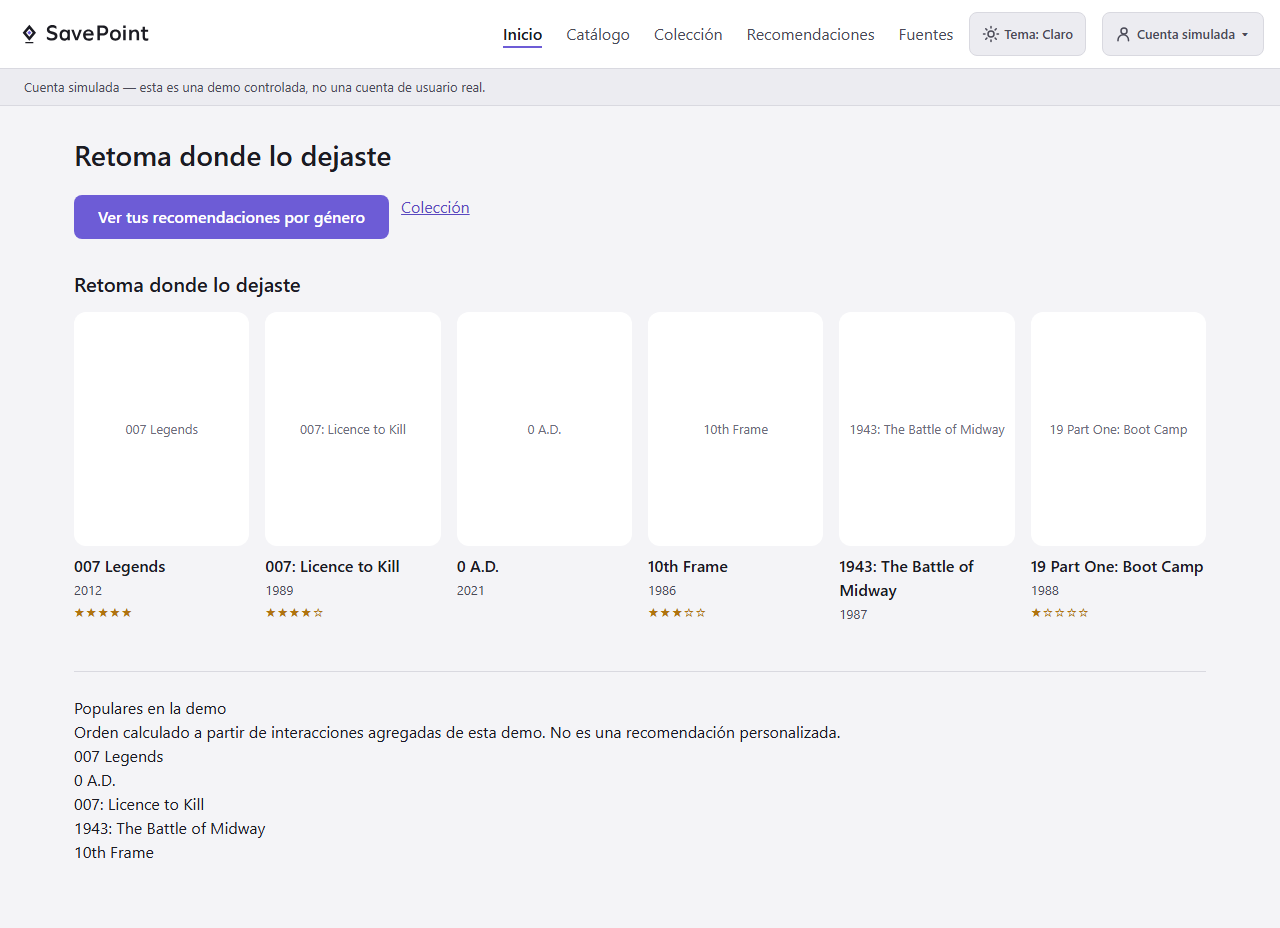
\includegraphics[width=0.85\textwidth]{figures/captura-home-claro.png}
    \caption{Página de inicio con tema claro.}
    \label{fig:ui-claro}
\end{figure}

\begin{figure}[H]
    \centering
    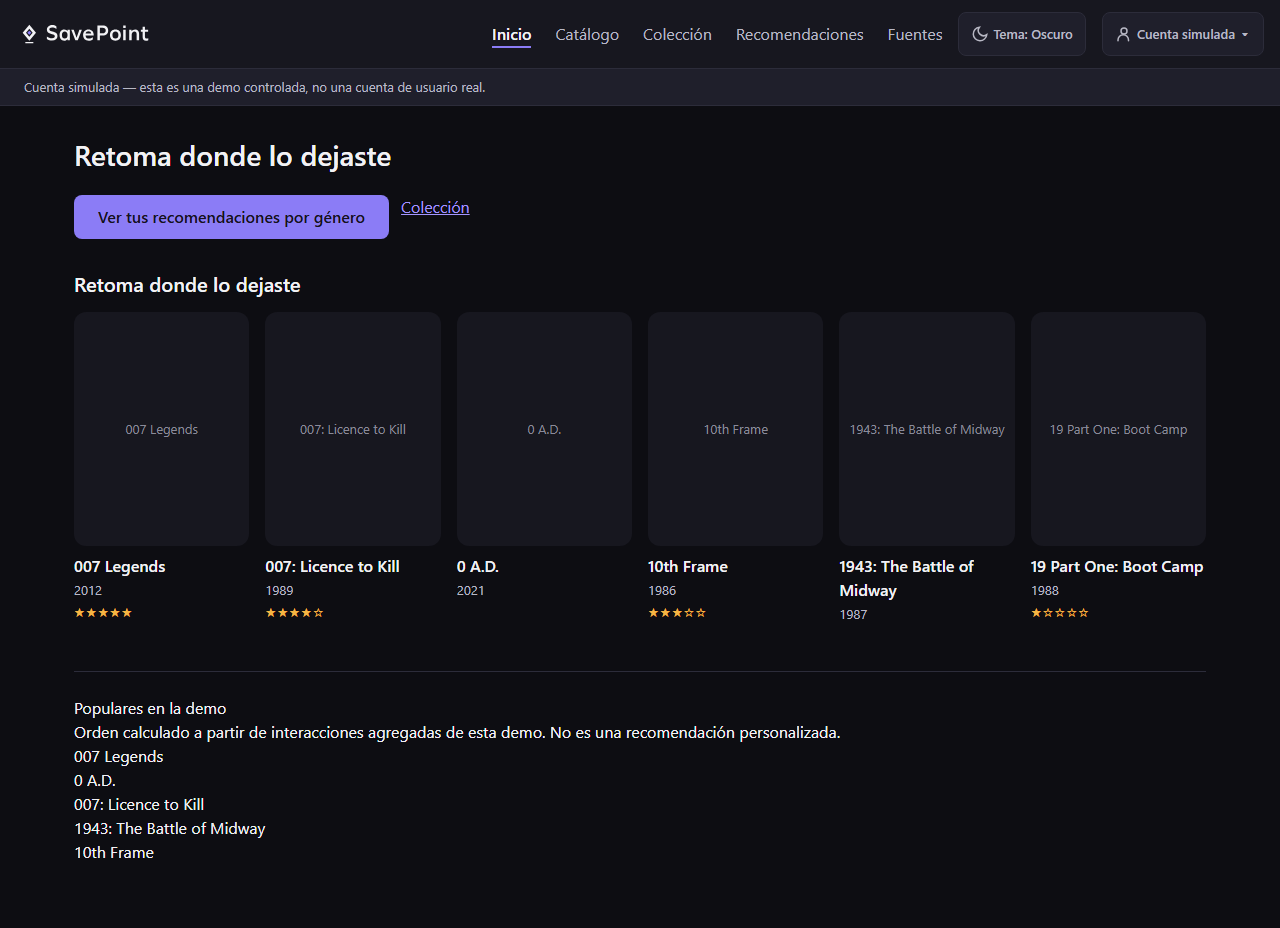
\includegraphics[width=0.85\textwidth]{figures/captura-home-oscuro.png}
    \caption{Página de inicio con tema oscuro.}
    \label{fig:ui-oscuro}
\end{figure}

El contrato de diseño incluye una matriz de cobertura por superficie, con filas para el
catálogo, el detalle, el registro y las recomendaciones, cada una con su verificación en
escritorio, en móvil y de accesibilidad. El Capítulo~\ref{cap:implementacion} describe las
rutas y los componentes concretos; la Sección~\ref{cap:pruebas} recoge su verificación.

\section{Diseño de los algoritmos de recomendación}\label{cap:algoritmos}\label{cap:nucleo-investigacion}

Esta sección detalla cómo SavePoint representa una obra y a una persona usuaria, qué señales
intervienen en la puntuación de una candidata, con qué fórmulas y pesos exactos se combinan esas
señales en cada uno de los dieciséis algoritmos comparados, qué respaldo en la literatura tiene cada
una de esas decisiones y cuáles se descartaron y por qué. El Capítulo~\ref{cap:resultados}
somete después esos algoritmos al protocolo de evaluación offline y presenta los resultados
obtenidos.

Conviene separar desde el principio dos planos que se confunden con facilidad. La literatura
avala las \emph{familias} de técnicas empleadas y los \emph{principios} de ponderación,
similitud, vecindad, hibridación, diversificación y medición; no convierte en constantes
universales los valores numéricos concretos que este proyecto fija. Los pesos por familia de
faceta, el parámetro \(\beta\) de la media F, el factor de contracción del rating, los pesos de
estado de biblioteca, el umbral de evidencia negativa, el \(\lambda\) de la reordenación y los
cortes \(K\) son decisiones explícitas de diseño para este corpus y este trabajo, tomadas y
documentadas como tales, no resultados heredados de una publicación. Cada apartado indica qué
parte pertenece a cada plano.

Los resultados publicados proceden de la ejecución \texttt{evaluation-400-test-2026-09-12-v15},
con el protocolo 15 y el \textit{feature set} \texttt{fs-v12-curated-tags-idf}. El código
vigente evolucionó después al protocolo 16 y al \textit{feature set}
\texttt{fs-v13-family-weighted-tags}, que corrigió el reparto de peso entre familias de
etiquetas descrito más abajo. Esa evolución permite describir con precisión la implementación
actual, pero no recalcula ni reinterpreta las métricas ya publicadas de v15, y así se indica en
cada cifra que proceda de una u otra versión.

\subsection{Representación de una obra y del perfil de la persona usuaria}\label{sec:alg-representacion}

La arquitectura de recomendación basada en contenido que sigue el sistema (describir cada ítem
con un conjunto de rasgos, construir un perfil de intereses a partir del historial de la
persona y comparar ambos para ordenar candidatas) es la formulación clásica de la familia,
descrita por Pazzani y Billsus~\cite{pazzani2007content}. Lo que este trabajo decide por su
cuenta es qué rasgos concretos describen un videojuego, cómo se curan y con qué intensidad
participa cada entrada de la biblioteca.

Una candidata para recomendar debe ser una obra gobernada del corpus, no contenido
descargable, publicada antes de la fecha de corte, con valoración externa disponible y al
menos cinco valoraciones agregadas; también se excluye cualquier obra que ya aparezca en la
biblioteca de la persona. Estas exclusiones impiden recomendar una posesión ya conocida,
lanzar contenido todavía no publicado o amplificar una nota sostenida por evidencia
insuficiente.

Cada obra se representa mediante un vector disperso de familias de facetas: etiquetas de
género y subgénero curadas, tema, característica, modo, franquicia, desarrollador y
plataforma. Los géneros y subgéneros forman el núcleo semántico de la representación; tema,
característica, modo, franquicia y desarrollador actúan como confirmaciones opcionales; la
plataforma expresa compatibilidad material más que afinidad de gusto. Las \emph{keywords},
perspectivas y modos crudos que ofrece la fuente de datos no se introducen directamente en el
vector: tienen ruido, sinónimos y semánticas heterogéneas, de modo que solo entran tras una
curación editorial que elimina duplicados y unifica niveles. Una faceta ausente en una obra se
omite sin más; el sistema nunca imputa ni redistribuye su peso a otra familia, porque hacerlo
premiaría la escasez de metadatos en lugar de ser neutral ante ella.

Dentro de cada familia, el peso de un valor concreto (por ejemplo, el género \texttt{rpg} o el
tema \texttt{cyberpunk}) se calcula con una frecuencia documental inversa suavizada, de modo
que un valor raro dentro de su propia familia pese más que uno común. El fundamento es la
ponderación estadística de términos y la representación vectorial dispersa de Salton y
Buckley~\cite{salton1988term}: los rasgos que aparecen en casi todos los documentos
discriminan poco, y los infrecuentes discriminan mucho. Desde la revisión \texttt{fs-v13}, cada
familia calcula su rareza sobre su propio universo de referencia, no sobre el corpus gobernado
completo: si \(N_f\) es el número de obras gobernadas con algún valor de la familia \(f\) y
\(df_t\) el número de esas obras que contienen el valor \(t\),

\begin{equation}\label{eq:idf}
idf(t) = \ln\!\left(\frac{N_f + 1}{df_t + 1}\right) + 1 ,
\end{equation}

con suavizado aditivo de \(1\) para mantener un valor finito incluso para un valor observado
en una única obra. La versión anterior, \texttt{fs-v12}, no separaba las familias: género,
subgénero, tema, modo y característica compartían un único presupuesto fusionado
(\(\mathtt{tag}=0{,}75\)) con un solo cálculo de IDF entre las cinco. Eso permitía que un
subgénero raro pesara más que el propio género por pura rareza estadística del conjunto
fusionado. Una primera corrección, renormalizar las cinco familias juntas sin separarlas,
se descartó porque terminaba premiando a las obras con menos metadatos en lugar de corregir el
sesgo. La solución adoptada en \texttt{fs-v13} fue separar cada familia en su propio cálculo de
IDF, con su propio universo de referencia \(N_f\) y su propio peso (\(\mathtt{tag}=0{,}60\),
que fusiona género y subgénero; \(\mathtt{theme}=0{,}20\); \(\mathtt{feature}=0{,}10\);
\(\mathtt{mode}=0{,}05\); \(\mathtt{platform}=0{,}05\)), de modo que la rareza de un valor se
mide siempre dentro de la población que realmente lo declara, no contra un denominador
compartido con familias de cobertura muy distinta. La fórmula procede de la literatura; el
cálculo de \(df\) sobre obras gobernadas, el suavizado y los pesos por familia son adaptaciones
reproducibles a este corpus. Franquicia
y desarrollador no usan IDF: si una obra declara \(k\) valores observados de esa familia, cada
uno pesa \(1/\sqrt{k}\), un reparto plano que evita premiar la rareza de un estudio o de una
saga, señales de cobertura desigual en las que una coincidencia rara diría más del catálogo que
del gusto de la persona.

Si \(T\) es el conjunto de valores que una obra declara en la familia \(f\), el peso de la
coordenada correspondiente a un valor \(t\) es

\begin{equation}\label{eq:facet-weight}
w(f{:}t) = W_f \cdot \frac{idf(t)}{\sqrt{\sum_{q \in T} idf(q)^2}} ,
\end{equation}

donde \(W_f\) es el peso fijo asignado a la familia \(f\) (Tabla~\ref{tab:pesos-familia}) y la
normalización L2 en el denominador, también procedente del modelo vectorial
clásico~\cite{salton1988term}, evita que una obra gane afinidad solo por declarar más valores
dentro de la misma familia. El reparto concreto de \(W_f\) es, en cambio, una decisión de
producto: prioriza la semántica de género sobre la compatibilidad de plataforma, que se
mantiene como una restricción y no como una afinidad. Igualar ambos pesos se consideró y se
descartó por ese mismo motivo.

\begin{table}[H]
\centering
\caption{Peso fijo \(W_f\) de cada familia de faceta en el vector de contenido,
\texttt{fs-v13}. Los valores son una decisión de diseño de SavePoint, no una constante de la
literatura.}\label{tab:pesos-familia}
\begin{tabularx}{\textwidth}{@{}Yr@{}}
\textnormal{Familia} & \textnormal{Peso \(W_f\)} \\
\hline
Etiqueta de género/subgénero (\texttt{tag}) & 0,60 \\
Plataforma (\texttt{platform}) & 0,05 \\
Tema (\texttt{theme}) & 0,20 \\
Característica (\texttt{feature}) & 0,10 \\
Modo (\texttt{mode}) & 0,05 \\
Franquicia (\texttt{franchise}) & 0,02 \\
Desarrollador (\texttt{developer}) & 0,015 \\
\end{tabularx}
\end{table}

El perfil de contenido de una persona usuaria se construye únicamente a partir de sus
entradas de biblioteca terminadas o en curso con valoración personal de al menos siete medios
puntos sobre diez; una entrada con valoración inferior a ese umbral no se añade al perfil
positivo, sino que alimenta un perfil de evidencia negativa aparte. Cada entrada \(i\) aporta
un peso de actividad \(entry\_weight_i = status\_weight_i + r_i^2\), donde \(status\_weight\)
vale 3 para una obra terminada, 2 para una obra en curso, 1 para pendiente y 0 para abandonada,
y \(r_i\) es la valoración personal normalizada a \([0,1]\). Elevar la valoración al cuadrado
hace que una nota alta cuente como evidencia bastante más intensa que una simplemente
positiva. Esta forma de modular la contribución de cada ítem del historial es la aplicación
directa del principio de perfil ponderado por interés de la familia basada en
contenido~\cite{pazzani2007content}; los valores 3, 2, 1 y 0 y el exponente cuadrático son
decisión local. El perfil es la media ponderada de los vectores normalizados de las entradas
elegibles, y no se vuelve a normalizar globalmente después; conserva así la intensidad relativa
acumulada de la biblioteca. Cuando una etiqueta se repite en al menos tres entradas de baja
valoración, se activa como evidencia negativa. Ese umbral de tres es deliberado: una
penalización sin umbral convertiría una única experiencia mal valorada en un rechazo estable,
que es precisamente el error que se quería evitar. Con menos de tres entradas positivas
elegibles, o sin ningún vector de features disponible, el sistema entra en un modo explícito de
historial insuficiente: no inventa un perfil ni recurre silenciosamente a la biblioteca de otra
persona; esa limitación queda declarada así en la respuesta.

\subsection{Similitud de contenido y señales escalares de la candidata}\label{sec:alg-similitud}

La similitud entre el perfil de una persona y una obra candidata no aplica el coseno
ciegamente sobre todo el vector. Para cada familia se calculan por separado la cobertura del
perfil y la precisión de la candidata: si \(P_f\) y \(C_f\) son los valores de perfil y
candidata en la familia \(f\), y \(O_f = P_f \cap C_f\) su solapamiento,

\[
coverage_f = \frac{\sum_{t \in O_f} P_f[t]}{\sum_{t \in P_f} P_f[t]}, \qquad
precision_f = \frac{|O_f|}{|C_f|} ,
\]

y ambas cantidades se combinan con una media \(F_\beta\) con \(\beta = 0{,}5\),

\begin{equation}\label{eq:fbeta}
F_{0.5} = \frac{(1+0{,}5^2)\;coverage \cdot precision}{0{,}5^2 \cdot precision + coverage} ,
\end{equation}

La media \(F_\beta\) como forma canónica de equilibrar precisión y cobertura con un único
parámetro procede de van Rijsbergen~\cite{vanrijsbergen1979information}; el valor
\(\beta = 0{,}5\) es la decisión local, y da más peso a la precisión de la candidata que a la
cobertura del perfil, de modo que una obra que declara muchos valores de una familia no gana
automáticamente por enumerar más. Se consideraron dos alternativas y se descartaron por
motivos concretos: una media aritmética simple favorece a las candidatas con más metadatos
declarados, y el coseno puro sobre el vector completo, aunque más habitual, resulta menos
separable a la hora de explicar por qué se recomienda una obra y más vulnerable a las
candidatas con muchas facetas.

Desde \texttt{fs-v13}, el núcleo renormalizado de la similitud se limita a las dos familias con
cobertura casi universal, etiqueta y plataforma, ponderadas exactamente con los pesos
\(W_{tag}=0{,}60\) y \(W_{platform}=0{,}05\) de la Tabla~\ref{tab:pesos-familia}:

\[
core = \frac{\sum_{f \in \{tag,\,platform\}} W_f \cdot F_{0.5,f}}{\sum_{f \in \{tag,\,platform\}} W_f \text{ activos}} .
\]

Las cinco familias restantes (tema, característica, modo, franquicia y desarrollador) suman
un bono de confirmación acotado, fuera de ese núcleo, que nunca resta ni se redistribuye
cuando una familia falta en cualquiera de los dos lados:

\begin{equation}\label{eq:bonus}
\begin{split}
bonus ={}& 0{,}20\,aff_{tema} + 0{,}10\,aff_{caracteristica} + 0{,}05\,aff_{modo}\\
      &+ 0{,}02\,aff_{franquicia} + 0{,}015\,aff_{desarrollador} ,
\end{split}
\end{equation}

con \(aff_f = \min\!\big(1,\, \sum_{t \in O_f} P_f[t] / \max_{t \in P_f} P_f[t]\big)\) y la
similitud final \(similarity = \min(1,\ core + bonus)\). Esta asimetría entre núcleo y bono es
deliberada: un tema, una saga o un estudio confirman un interés ya observado en el género o la
plataforma, pero no deben sustituir esa similitud semántica ni inflarla artificialmente cuando
falta información secundaria. Situar franquicia o desarrollador en el núcleo se descartó por su
cobertura desigual y por el riesgo de recomendar por coincidencia superficial de editor más que
por afinidad real. El coseno completo sobre el vector no desaparece: se reserva para medir la
redundancia entre recomendaciones y la diversidad intra-lista de las variantes con
reordenación, donde su interpretación geométrica directa sí es exactamente la propiedad
necesaria.

La calidad externa de una candidata no usa su valoración agregada en bruto, sino que se
estabiliza con contracción (\emph{shrinkage}) bayesiana hacia la media del corpus, para que una
nota extrema sostenida por pocas observaciones no domine el resultado. El fundamento es el
principio de Empirical Bayes: las observaciones escasas se contraen hacia un prior común para
reducir la varianza del estimador~\cite{efron2010large}. Con \(n\) valoraciones observadas,
prior del corpus \(\mu\) (la media de valoraciones ponderada por su propio volumen de votos) y
un parámetro de contracción \(m=25\),

\[
rating_{bayes} = \frac{n \cdot rating + m\,\mu}{n+m}, \qquad
rating_{final} = \left(\frac{rating_{bayes}}{100}\right)^{2} \cdot \frac{n}{n+m} .
\]

El valor \(m=25\), el exponente cuadrático sobre la nota normalizada y el factor de confianza
\(n/(n+m)\) son, de nuevo, decisiones locales: el cuadrado separa mejor a las candidatas de
calidad alta y el factor de confianza penaliza de forma explícita el volumen de evidencia, no
solo la nota media. Usar la valoración en bruto se descartó por el sesgo evidente de las notas
extremas con poca evidencia, y volver a multiplicar por el volumen de votos también, porque ese
volumen ya participa una vez dentro de la propia contracción. Cuando una candidata no tiene
valoración externa propia observada, el sistema recurre a la mediana de valoración de sus
etiquetas curadas y marca el resultado como una aproximación, sin presentarlo como una
observación real.

La popularidad externa (\emph{PopScore}) tampoco usa el valor bruto de la fuente de datos: su
escala es larga y arrastra un sesgo de popularidad conocido, así que cada una de sus cuatro
primitivas se transforma con \(\log(1+x)\) y después se convierte en un percentil de rango
dentro del snapshot congelado, combinándose como \(PopScore = 0{,}40\,\text{Visitas} +
0{,}25\,\text{Jugando} + 0{,}25\,\text{Jugado} + 0{,}10\,\text{Quiere jugar}\). Si falta
cualquier primitiva, no existe composición observada y las variantes que la consumen aplican un
suelo explícito de cero, marcado como tal, sin redistribuir el peso que le correspondía. La
recencia, por último, solo es estimable para una obra con fecha de lanzamiento no futura: con
\(year\_gap\) el número de años naturales transcurridos desde su publicación hasta la fecha de
corte, \(recency = 0{,}35^{\,year\_gap}\), de modo que una obra del año del corte vale
\(1{,}0\), una del año anterior \(0{,}35\) y así sucesivamente. Se eligió una base geométrica
sobre años naturales en lugar de una semivida diaria porque esta última es menos interpretable
y depende del día exacto del corte, lo que la haría frágil ante una repetición del experimento
en otra fecha.

\subsection{Las tres familias y sus dieciséis variantes}\label{sec:alg-familias}

Con la afinidad de contenido \(C\), la calidad \(R\), la popularidad \(P\), la evidencia
negativa \(N\) y la recencia \(X\) ya definidas, la Tabla~\ref{tab:variantes-contenido} recoge
la fórmula exacta de las diez variantes basadas en contenido. Todas comparten el mismo conjunto
de candidatas, el mismo vector de features y el mismo perfil de usuario; lo único que cambia
entre ellas es cómo combinan sus señales, precisamente para que la comparación aísle esa
decisión de diseño y no otra.

\begin{table}[H]
\centering
\caption{Fórmula de combinación de las diez variantes basadas en contenido.}\label{tab:variantes-contenido}
\small
\begin{tabularx}{\textwidth}{@{}>{\ttfamily\raggedright\arraybackslash}p{0.48\textwidth}>{\raggedleft\arraybackslash}X@{}}
\textnormal{Algoritmo} & \textnormal{Fórmula} \\
\hline
content-cbf-weighted-v1 & \(S = 0{,}70\,C + 0{,}30\,R\) \\
content-cbf-multiplicative-v1 & \(S = C \cdot R\) \\
content-cbf-twostage-v1 & \(b=\min(4,\lfloor 5C\rfloor);\ S = b + R/6\) \\
content-cbf-neg-v1 & \(S = \max(0,\ 0{,}70C + 0{,}30R - N)\) \\
content-cbf-weighted-pop-v1 & \(S = 0{,}55C + 0{,}25R + 0{,}20P\) \\
content-cbf-multiplicative-pop-v1 & \(S = C \cdot R \cdot (0{,}80 + 0{,}40P)\) \\
content-cbf-twostage-pop-v1 & \(b=\min(4,\lfloor 5C\rfloor);\ S = b + (0{,}80R+0{,}20P)/6\) \\
content-cbf-neg-pop-v1 & \(S = \max(0,\ 0{,}55C + 0{,}25R + 0{,}20P - N)\) \\
recency-v1 & \(S = 0{,}20C + 0{,}20R + 0{,}20P + 0{,}40X\) \\
content-cbf-mmr-v1 / -pop-v1 & MMR sobre Weighted / Weighted-Pop \\
\end{tabularx}
\end{table}

La existencia de estas diez variantes no responde a un afán de acumular algoritmos, sino al
diseño experimental: cada una aísla una única decisión de combinación manteniendo constantes
las candidatas, las features y los snapshots, de modo que una diferencia de resultado se pueda
atribuir a esa decisión concreta. \texttt{content-cbf-weighted-v1} actúa como referencia del
grupo porque sus pesos son explícitos y su comportamiento es fácil de explicar: el contenido
domina la puntuación y la calidad ordena dentro de un mismo nivel de afinidad. La variante
multiplicativa exige afinidad y calidad simultáneamente, sin que una compense a la otra. La de
dos etapas usa la afinidad para asignar una banda discreta y solo desempata dentro de ella con
la calidad, de modo que una nota alta nunca rescata una afinidad baja. La negativa resta la
evidencia de rechazo acumulada sobre las mismas etiquetas. Las cuatro variantes con sufijo
\texttt{-pop} repiten exactamente esas combinaciones incorporando además un veinte por ciento
de PopScore, con el resto de pesos reescalados para que la suma se mantenga acotada; en la
multiplicativa, un PopScore nulo produce un factor \(0{,}80\) y uno máximo un factor
\(1{,}20\), un ajuste acotado y nunca una sustitución de la afinidad de contenido.
\texttt{recency-v1} reparte su peso entre las cuatro señales con un cuarenta por ciento para la
novedad, lo que la convierte en una variante de descubrimiento sin abandonar del todo la
personalización.

Fuera de la familia de contenido, \texttt{cf-user-knn-v1} implementa el filtrado colaborativo
por vecindad de usuarios en la forma que introdujeron Resnick y otros en
GroupLens~\cite{resnick1994grouplens} y que sistematizaron Herlocker y
otros~\cite{herlocker2004evaluating}: similitud entre personas calculada sobre las obras que
ambas han valorado, valoraciones centradas por la media de cada persona y predicción por
agregación ponderada de las desviaciones de los vecinos. Las decisiones locales son el mínimo
de dos obras co-valoradas para considerar fiable una vecindad y el máximo de veinte vecinos con
similitud positiva. Es explicable por los vecinos y las obras que comparten, pero sufre
arranque en frío: con historial escaso, o sin vecindad suficiente, no puede inferir una
preferencia colaborativa fiable. Se descartó implementar en su lugar un colaborativo por
vecindad de ítems porque exige construir una matriz ítem-ítem y descansa sobre otra hipótesis
de generalización, mientras que la vecindad de usuarios resulta más legible con el rating
explícito disponible en este corpus.

El híbrido responde al argumento de Burke~\cite{burke2002hybrid}: combinar fuentes
complementarias permite aprovechar las ventajas de cada una y compensar sus debilidades. Su
combinación es \(H(i) = 0{,}60\,\mathit{Weighted}(i) + 0{,}40\,\mathit{CF}(i)\); si el
componente colaborativo no dispone de historial suficiente, el híbrido conserva la relevancia
de contenido y declara el \emph{fallback} en lugar de penalizar artificialmente a una persona
nueva. El reparto 0,60/0,40 es en sí mismo una decisión local sujeta a evaluación, no una regla
tomada de la literatura.

Las dos variantes con reordenación por diversidad aplican \emph{maximal marginal relevance}
tal como lo formularon Carbonell y Goldstein~\cite{carbonell1998mmr}: recorren un conjunto de
tamaño \(\max(100, 5K)\) y en cada posición eligen la candidata que maximiza
\(\lambda\,Rel(i) - (1-\lambda)\max_{j \in S} cosine(i,j)\), con \(Rel(i)\) la relevancia ya
calculada y \(S\) la lista parcial ya elegida. El valor \(\lambda = 0{,}80\) y el tamaño del
conjunto son decisiones locales. La motivación de fondo es la advertencia de McNee, Riedl y
Konstan~\cite{mcnee2006accurate} y el marco de medición de Vargas y
Castells~\cite{vargas2011rank}: la exactitud no agota la utilidad de una recomendación, y
diversidad, novedad y cobertura deben medirse aparte en lugar de quedar escondidas dentro de la
puntuación. Por eso la diversificación se implementó como una capa de reordenación explícita y
no como un término más dentro de los pesos de afinidad, ni como una optimización multiobjetivo
del propio \emph{score}: separarlas permite estudiar el compromiso entre relevancia y
redundancia en lugar de ocultarlo.

\subsection{Variantes publicadas en la aplicación}\label{sec:alg-publicadas}

De las dieciséis variantes, la aplicación web publica solo tres: \texttt{content-cbf-weighted-v1},
\texttt{content-cbf-mmr-pop-v1} y \texttt{recency-v1}. Cada una responde a un criterio distinto.
La primera es la referencia de la familia de contenido: el contenido domina la puntuación y la
calidad externa ordena dentro de un mismo nivel de afinidad. La segunda añade popularidad y una
reordenación por diversidad, para que la lista no repita variaciones del mismo juego. La
tercera favorece los títulos recientes y actúa como variante de descubrimiento. La selección es
una decisión de diseño de producto: ofrecer a la persona usuaria dieciséis listas con resultados
muy parecidos entre sí no aporta valor y empeora la experiencia, y mantener un \textit{worker}
activo por cada variante supone un coste de recursos que no se justifica. Las demás variantes
se conservan en el laboratorio de evaluación, donde cumplen su función, que es compararlas bajo
un mismo protocolo, y no afectan a esta selección: el Capítulo~\ref{cap:resultados} evalúa las
dieciséis.

\subsection{Alternativas descartadas y su justificación}\label{sec:alg-alternativas}

Las familias implementadas son interpretables y adecuadas para una población controlada, pero
no agotan el espacio de recomendación. La Tabla~\ref{tab:alternativas} recoge las alternativas
que se consideraron de forma explícita, con su respaldo en la literatura cuando lo tienen, y el motivo
por el que no se adoptaron en esta versión.

\begin{table}[H]
\centering
\caption{Alternativas consideradas y motivo de exclusión.}\label{tab:alternativas}
\tablecompact
\renewcommand{\arraystretch}{1.25}
\begin{tabularx}{\textwidth}{@{}>{\raggedright\arraybackslash}p{0.43\textwidth}Y@{}}
\textnormal{Alternativa} & \textnormal{Motivo de exclusión} \\
\hline
Factorización matricial (ALS, BPR)~\cite{koren2009matrix} & Añade entrenamiento, factores latentes e hiperparámetros; dificulta atribuir un resultado a una señal concreta sobre población sintética \\
Redes neuronales, \textit{embeddings} o modelos de lenguaje & Coste, opacidad y requisitos de datos no justificados por el objetivo del trabajo \\
Modelos de grafos o secuenciales & El historial disponible no sostiene una hipótesis temporal que justifique esa complejidad \\
Colaborativo por vecindad de ítems & Exige matriz ítem-ítem y otra hipótesis de generalización; user-KNN es más legible con rating explícito \\
Coseno puro como similitud principal & Menos separable en las explicaciones y más vulnerable a candidatas con muchas facetas \\
Media aritmética en lugar de \(F_{0.5}\) & Favorece a las candidatas que declaran más metadatos \\
Rating externo en bruto & Sesgo de las notas extremas con poca evidencia; la contracción bayesiana lo corrige \\
PopScore en bruto & Escala larga y sesgo de popularidad; se normaliza por percentil dentro del snapshot \\
Optimización multiobjetivo del \emph{score} & Escondería la diversidad dentro de los pesos de afinidad en lugar de permitir estudiarla \\
Métricas de error sobre la nota predicha & Miden predicción de valoración, no calidad del orden de la lista~\cite{cremonesi2010performance} \\
\end{tabularx}
\end{table}

Estas exclusiones son decisiones de alcance y de validez, no afirmaciones de que los métodos
descartados sean universalmente peores. La factorización matricial, en particular, es una
alternativa reconocida y competitiva en recomendación colaborativa~\cite{koren2009matrix}; no
se incorpora porque el objetivo de este trabajo exige comparar señales legibles sobre una
población controlada, y un modelo de factores latentes introduciría entrenamiento y grados de
libertad que harían mucho más difícil atribuir una diferencia de resultado a una señal
concreta. Cualquiera de ellas podría evaluarse en una extensión del trabajo, pero exigiría una
variante versionada, nuevos controles de datos y una comparación bajo el mismo protocolo.

\section{Diseño del laboratorio de evaluación}\label{sec:dis-laboratorio}

El laboratorio se diseñó como una tubería fuera de línea, separada de las peticiones de
usuario. Su entrada no es el valor mutable de \texttt{GameWork.total\_rating}, sino una
pareja de versión de corpus y snapshot de valoraciones. A partir de ella, el runner resuelve
la partición de usuarios, construye el manifiesto de candidatos de cada usuario y ejecuta
las variantes sobre la misma entrada. El artefacto resultante debe conservar la versión del
código, la huella del protocolo, las semillas, la huella del manifiesto y las métricas por
usuario y por $k$. La Figura~\ref{fig:pipeline-evaluacion} resume esa tubería.

\begin{figure}[htp]
    \centering
    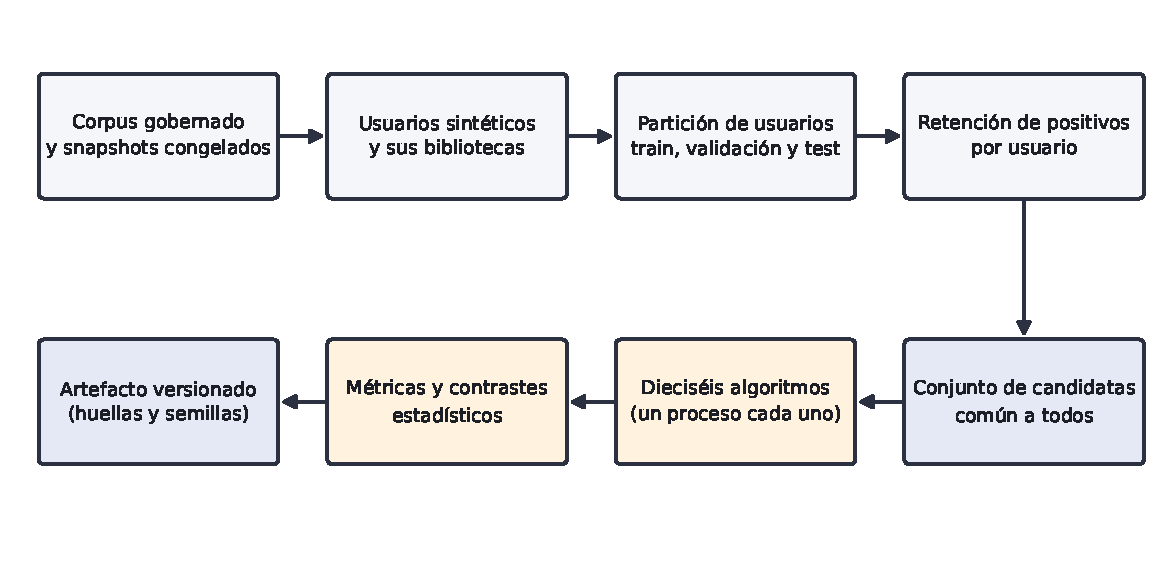
\includegraphics[width=0.9\textwidth]{figures/pipeline-evaluacion.pdf}
    \caption{Tubería de la evaluación offline, de los datos congelados al artefacto versionado.}
    \label{fig:pipeline-evaluacion}
\end{figure}

La aplicación \texttt{evaluation} separa cuatro responsabilidades. El cargador del
protocolo valida las claves, el tamaño de la rejilla y el consumo único del test. El módulo
de particiones selecciona la obra relevante retenida y comprueba que train, validation y test
sean conjuntos disjuntos y completos. El módulo de métricas calcula P@K, R@K, nDCG@K y MAP@K
con fórmulas escritas y probadas en el proyecto. Por último, el runner orquesta los algoritmos
y escribe un artefacto JSON con sus huellas y resultados.

Todas las variantes comparten el conjunto de candidatos, la semántica de exclusión y el DTO
versionado; el modelo de contenido que usan es el descrito en la
Sección~\ref{cap:algoritmos}. Las explicaciones no generan texto libre: devuelven una tabla
determinista de contribuciones por faceta, el valor del término de rating y si se usó el
fallback. El parámetro \texttt{algorithm\_id} solo puede seleccionar identificadores de una
allowlist, nunca una función o importación dinámica.

Este capítulo ha descrito cómo se diseñaron la plataforma, los algoritmos de recomendación y el
laboratorio que los compara. El capítulo siguiente describe su implementación.
